\documentclass[]{template}    
\begin{document}
\section{生成事件描述}

\subsection{本章概述}
在前两章,我们首先验证了事件描述对事件成功的影响,并通过事件属性预测了事件结果,以及衡量了事件描述与事件参与人数的关系。后者对于事件组织者尤为重要,因为一个组织者总是会关心他的活动会有多少人参加。而另一个事件组织者十分感兴趣的话题是他该如何写出好的事件描述。因此,如果能够根据历史数据,来自动生成一些事件描述供组织者参考,是十分有意义的。

本章在上一章的基础上,设计了一个生成模型(\textit{generator}),用来生成事件描述。在考察了诸多文本生成模型后,我们在本文使用了变分自编码器\cite{kingma_auto-encoding_2013,bowman_generating_2015}(\textit{variational autoencoder})。这里使用变分自编码器的原因是因为我们希望文本在编码空间内服从我们期望的分布,具体的来说,我们希望每段文本的隐编码的周围是连续的,同时不同文本的隐编码在隐空间间也是连续的,这样的话可以避免传统编码器所带来的一些问题,比如样本在隐空间的分布不连续,导致只无法在隐空间采样来生成文本。然后我们使用上一章设计的基于GRU的神经网络作为判别器(\textit{discrimitor}),组成一个生成对抗网络\cite{goodfellow_generative_2014}。由于在训练时借鉴了强化学习中的策略梯度下降(\textit{policy gradient}),因此我们将其命名为GAN\_PG,通过设计合理的奖励函数,来训练生成器生成好的事件描述。

本章的结构如下:首先我们会详细介绍文本生成模型的设计和训练过程,然后我们会对GAN\_PG中使用的生成模型以及其奖励函数进行详述,最后我们会在真实的\textit{meetup}数据集上给出实验结果。

\subsection{事件描述生成模型}
\subsubsection{循环神经网络语言模型}
循环神经网络语言模型(\cite{RNNLM})是目前十分流行的一种语言模型。在生成句子时,RNNLM仅根据当前隐层的状态给出下一个词的概率分布,而不是其他假设。而RNN模型本身又十分强大,几乎可以拟合任何分布。而自然语言在某种程度上又可以看成一个概率模型,每一个词出现的概率都由之前已出现的词决定,因此,只要有训练数据,RNNLM就可以很好的对复杂文本序列建模。反应在实验中就是其生成的文本十分像它的训练数据,例如如果我们使用莎士比亚的文章作为训练数据,那么其生成文本读起来也像莎士比亚。这种性质也让它在文本生成器中得到了广泛应用,几乎所有的序列到序列(\textit{seq2seq})模型中的解码器(\textit{decoder})都采用了RNNLM。本文也不例外。
\subsubsection{变分自编码器}
RNNLM在生成文本序列中的某一个词时,完全依赖于之前输入的词和隐状态。而在实现中,通常会使用一个特殊符号来作为每一句的开头,因此,RNNLM生成的文本序列完全依赖于其刚开始时的隐状态。所以如何提供合适的隐状态来使生成的句子符合预期,就显得尤为重要了。一个解决方案是使用第二章提到的GRU编码器。编码器首先将输入序列编码到一个隐空间,然后使用一个前向神经网络将这条编码转换成RNNLM初始化的隐状态。但是这样做有一个非常明显的缺陷:我们无法控制输入样本经过编码器编码后在隐空间中的分布。在原空间相似的两个文本序列在编码后它们所对应的隐向量可能并不相近。这显然不是我们期望的。另一方面是,GRU在编码过程中,是直接算出对应文本序列的隐编码,而非采样获得,这就导致了隐编码在隐空间中是不连续的,换而言之,在隐空间中可能只有几个点有意义。因此,在这里仅依靠GRU编码器是不够的。但是我们可以使用变分编码器,它是传统的RNN编码器的改进型,它对隐空间中的编码\(\overrightarrow{z}\)加入了先验分布,并在目标函数中通过kl散度来缩小实际分布和先验分布的距离,以此来强迫编码器学到合适的编码方式。同时,它通过采样来生成编码,这也就保证了隐编码周围的点也都是有意义的。变分自编码器的损失函数$L_i(\theta,\phi)$如公式(\ref{3-1})。
\begin{equation}\label{3-1}
    L_i(\theta,\phi)=-E_{z\sim q_\theta(z|x_i)}[\log p_\phi(x_i|z)]+KL (q_\theta(z|x_i)||p(z))
\end{equation}
可以看出,其损失函数由两部分构成,第一部分是负对数似然损失函数,用来缩小输入序列和输出序列的差异。第二个部分则是kl散度,其中$q_\theta$为编码器,$p(z)$为对隐编码$z$的先验分布。

\subsubsection{事件描述生成模型}
我们使用了\cite{bowman_generating_2015}中的VAE结构,如图\ref{f3-2}所示。在编码器和解码器的选择上,我们都使用了单层GRU。在实现过程中,我们使用$0-1$高斯分布作为隐编码的先验分布。同时使用了重采样\cite{kingma_auto-encoding_2013}的技巧,这样我们便可以用反向传播来训练我们的网络:在抽样的时候,我们不直接对隐编码进行采样,而是通过两个线性神经网络获得当前编码的平均值$\bar{u}$标准差$\bar{v}$,然后通过公式(\ref{3-2})获得隐编码,其中$\bar\epsilon \sim Normal(0,1)$。
\begin{figure}[htb]\label{f3-2}
    \centering
    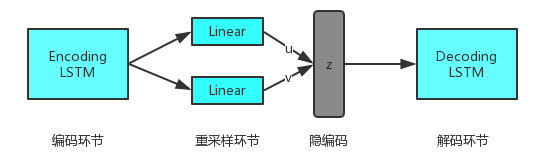
\includegraphics[width=11.3cm]{vae.png}
    \caption{事件描述生成模型的核心结构,蓝色为神经网络,灰色为向量,输入为预先训练的词向量。在编码环节完成后,LSTM的隐状态将分别输入到两个线性网络中,得到隐编码分布的平均$\bar{u}$和方差$\bar{v}$,然后通过采样获得隐编码,并将其输入解码环节。}
\end{figure}
\begin{equation}\label{3-2}
    z=\bar{u}+\bar{v}\odot \bar\epsilon
\end{equation}

至于如何使用前半段编码结果来初始化解码器中的隐状态,我们尝试了三种方法1)将隐编码连接在解码器的输入词向量的最后。2)将隐编码通过一个前向网络转换成解码器的隐状态向量,并用它直接初始化后者。3)两者皆做。在实际运用过程中,我们发现这三种方法并没有很大的差别,因此最终我们采用了第一种方案。

在实际的训练过程中,为了防止损失函数中KL散度降为0,我们还参考了\cite{bowman_generating_2015}中所采用的策略:在训练刚开始时设置KL散度项的权重为零,然后慢慢升到一。这样训练过程其实就分成了两个阶段:第一个阶段,编码器从文本序列中学到尽可能多的信息,但不保证分布符合先验分布。第二阶段,通过增加KL散度项的权重,强迫编码器编得的隐编码尽可能接近先验分布。

\subsection{GAN\_PG}
通过前文的事件描述生成器,我们可以生成读上去通顺的事件描述。只要训练数据是文法通顺的句子,那么输出也会是文法通顺的句子。我们有两种方式可以获得事件描述:一种是在隐编码空间里面随机采样。这样生成的事件描述文法通顺,但无法保证语义上的一致。另一种是在已知事件描述的隐编码周围采样,由于采用了变分自编码器,相似的文本序列的隐编码在隐空间中也是相近的。因此,如果我们采用第二种方法,仅在已知事件描述隐编码的周围采样,我们便可以获得和已知事件描述在文法上一致的新的事件描述。如果我们能找到一种方法,使每次的改变都往我们期望的方向上发生,便可以起到改进事件描述的作用,正如\cite{noauthor_sequence_nodate}中做的一样。而借助上一章的预测器,我们可以预测新的事件描述的参与人数。而通过设计合理的奖励函数,我们可以让解码器学到如何生成能够在预测器上获得高分的文本序列。但这样做有一个问题:我们不能保证预测器是可靠的,即在预测器上获得高分的文本序列可能并不符合我们的期望,因此在训练生成器的同时,我们还要对预测器进行训练,使之能正确的区分真正的样本和生成的样本,这便是此处用到生成对抗网络的原因了。
\subsubsection{生成对抗网络简介}
生成对抗网络(\textit{Generative Adversarial Net}\cite{goodfellow_generative_2014})是Goodfellow于2014年提出的。它包含生成(\textit{generator})模型和判别(\textit{discrimitor})模型。在训练过程中,生成模型的目标是生成能够让判别模型无法分辨出其和真实数据的区别样本,而判别模型的训练目标则是将生成模型生成的假样本从真实样本中区分开来。在标准的生成对抗网络中,我们最大化判别模型正确分类的概率,同时最小化生成模型所生成的样本被判别器正确分类的概率,目标函数见\ref{3-3}。
\begin{equation}\label{3-3}
    \mathop{min}_G \mathop{max}_D V(D,G)=E_{x\sim data}[\log D(x)]+E_{x'\sim G_\theta}[\log(1-D(x')]
\end{equation}

其中,$D,G$分别表示判别和生成模型,$data$表示真实数据集。$G_\theta$表示生成模型产生的假数据。
\subsubsection{GAN\_PG}
GAN\_PG的生成模型为本章第二节介绍的事件描述生成模型,判别模型为上一章介绍的带GRU的神经网络。判别模型的损失函数为最小化公式(\ref{3-4})式(即在公式(\ref{3-3})前加上负号)。
\begin{equation}\label{3-4}
    \mathop{min}_D-E_{x\sim data}[\log D(x)]-E_{x'\sim G_\theta}[\log(1-D(x')]
\end{equation}
生成模型的损失函数为最大化公式(\ref{3-5})。其中$G_\theta,D_\sigma$分别为生成模型和判别模型,公式(\ref{3-5})的前半部分为在隐编码$z$和已生成的序列$y_{0:t-1}$下,生成当前$y_t$的概率。公式(\ref{3-5})的后半部分为生成模型生成$y_t$在判别模型所获得的评分。最大化公式(\ref{3-5})即最大化生成模型在生成序列的每一步中所获得的评分。
\begin{equation}\label{3-5}
pg\_loss=\mathop{min}\sum_{\substack{t}}-\log G_\theta (y_t|z,y_{0:t-1})*D_\sigma (y_t,y_{0:t-1})
\end{equation}

接下来的问题是如何衡量生成模型所生成的每一步获得的评分。因为判别模型只有在生成模型生成完整个序列以后,才能对该序列评分,而公式(\ref{3-5})所要求的是实时的评分。在本文中,参考\cite{yu_seqgan:_2016}中所用的方法,我们使用了策略梯度来设计损失函数:对于$t$时刻所生成的序列$y_t$,我们使用了策略网络$G_\theta$(即当前生成模型)通过蒙特卡洛搜索算法对接下来$T-t$项(T为序列长度)进行采样,即公式(\ref{3-6})。
\begin{equation}\label{3-6}
    \{y_0,y_1,\dotsb,y_T\}=\mathrm{MC}^{G_\theta}(y_{0:T})
\end{equation}

其中$y_{0:t}$为当前状态,$y_{t+1:T}$为基于当前生成器装态采样的结果。为了获得更准确的结果,我们可以将上述过程重复数次,取平均。经过改进的生成模型目标函数如公式(\ref{3-7})。
\begin{equation}\label{3-7}
D_\sigma(y_t,y_{0:T-1})\sim 
\begin{cases}
    D_\theta(y_{0:T-1}) & \text{if } t =T-1 \\
    \mathrm{E}(D_\theta(y_{0:t-1}:y_t:y_{t+1:T-1})),y_{t+1:T-1}\sim \mathrm{MC}^{G_\theta}(y_{0:t}) & \text{if }t<T-1
\end{cases}
\end{equation}

在确定了判别器,生成器和其分别的目标函数后,我们通过算法公式(\ref{s3-1})来训练GAN\_PG。
\begin{table}[htbp]
    \label{s3-1}
    \begin{center}
        \begin{tabular*}{.75\linewidth}{p{0.75\linewidth}}
\toprule
            算法一、训练GAN\_PG \\
\midrule
\begin{minipage}[t]{\linewidth}
\begin{enumerate}[itemsep=-10pt]
    \item 预训练生成模型
    \item 预训练判别模型
    \item \textbf{repeat}
    \item \quad \textbf{for} g-step \textbf{do}
    \item \quad \quad 使用$G_\theta$生成序列$S_{0:T}$
    \item \quad \quad 使用公式(\ref{3-5})计算目标函数
    \item \quad \quad 更新参数$\theta$
    \item \quad \textbf{end for}
    \item \quad \textbf{for} d-step \textbf{do}
    \item \quad \quad 采集\textbf{n}个负样本,\textbf{m}个正样本
    \item \quad \quad 计算与目标的均方误差
    \item \quad \quad 更新参数
    \item \quad \textbf{end for}  
    \item \textbf{end for}
\end{enumerate}
\end{minipage}\\
\bottomrule
        \end{tabular*}
    \end{center}
\end{table}

\subsection{实验}
在本小节,我们将在真实的数据集上验证我们的方法,本章采用的数据集和第一,第二章相同,在此不多做介绍。本章的结构将分为两个部分,第一部分阐述事件描述生成模型,即生成模型的预训练,第二部分描述判别模型和GAN\_PG的训练。
\subsubsection{训练事件描述生成模型}\label{train_generator}
\paragraph{训练细节}
在训练事件描述生成器时,我们要保证其目标函数公式(\ref{3-1})的两部分处在合适的平衡状态。因为一方面我们前半项越小越好,另一方面我们又希望后半项较小又不太小。保证前半项足够小是为了缩小和训练样本的距离,后半项相对较小是为了让其隐编码服从特定分布,但如果后半项太小,则不同训练样本的隐编码过于相似(都接近0-1高斯分布),也失去了编码器的意义。所以我们使用文提及的方法,在训练过程中让后半项的权重为0,先训练前半项,再慢慢将后半项的权重增加,以训练后半项。在实现过程中,我们用了公式(\ref{3-8})来调整后半项的权重,同时为了使后半项值能稳定在合适的范围,我们将前半项的系数设置为79。训练的前半项,后半项以及$\mathrm{KL\_Weight}$的变化图如图\ref{f3-2}。接下来,我们将对训练好的生成器进行实验。我们将做两个实验:对已知样本的采样和随机采样。

\begin{figure}[htb]
    \centering
	\begin{subfigure}{.4\textwidth}
		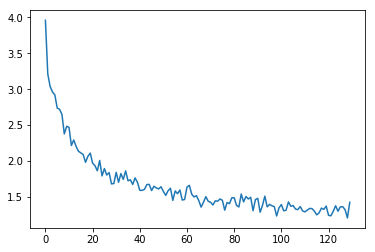
\includegraphics[width=\textwidth]{ce.png}
		\caption{前半项($\mathrm{NLL}$)变化}
	\end{subfigure}
	\begin{subfigure}{.425\textwidth}
		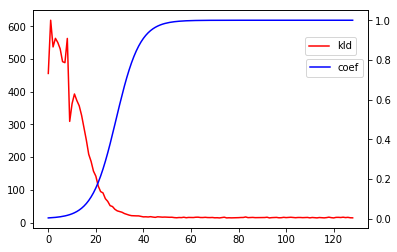
\includegraphics[width=\textwidth]{ceof.png}
		\caption{后半项($\mathrm{KL}$距离)及其系数变化}
    \end{subfigure}
    \caption{事件描述生成模型训练过程中,目标函数变化曲线,$x$轴为循环次数,最终$\mathrm{KL}$稳定在7附近}
    \label{f3-2}
\end{figure}

\begin{equation}\label{3-8}
    \mathrm{KL\_Weight}=\frac{\tanh\frac{i-3000}{1000}+1}{2}
\end{equation}

\paragraph{对已知样本采样}  
在本节中,我们将对已知样本的隐编码$z \sim \mathrm{p}(z|x)$进行采样,其中$x$为已知的文本序列,即事件描述。$\mathrm{p}(z|x)$为编码过程。我们通过公式(\ref{3-2})进行采样。通过此举,我们可以对生成器认为的相似的句子有个大概的了解。实验结果如表\ref{t3-2}所示。 
\begin{table}[htb]
    \center
    \caption{\label{t3-2}对已知样本采样的结果}
    \begin{tabular*}{\linewidth}{p{0.2\linewidth}p{0.8\linewidth}}
\toprule
样本一 & we are meeting at the actual merry go round <ukn> . \\
对隐编码解码 & we will be meeting at the corner of the park entrance .\\ 
采样一 & we will be meeting in the back room , and then the <ukn> will be on the right hand side of the stage .\\
采样二 & we are going to have a great time of year 's theme for the day . \\
采样三 & we will be meeting at the end of the day before the show . \\
\midrule
样本二 & we 'll be there the whole night . \\
对隐编码解码 & we will have a dj spinning the best of the night !\\ 
采样一 & we 're going to have a great turnout .\\
采样二 & the presentation will be on the right side of the road .\\
采样三 & after the concert we 'll have a chance to visit the bars in the park . \\
\bottomrule
    \end{tabular*}
\end{table}
\paragraph{随机采样}
本节中,我们将对未知的隐编码进行采样,同时检验在编码空间中相邻点的编码结果的语义一致性和文法一致性。我们先在隐空间中进行采样,获得隐编码$z_1,z_2 \sim \mathrm{Normal}(0,1)$,然后我们在两点间进行线性插值,获得编码集合$\{z_i\} = t*z_1+(1-t)*z_2 ,\mathrm{for}\ t \in [0,1]$。随后我们再对集合$\{z_i\}$进行采样,采样结果见表\ref{t3-3}。借助此举,我们可以了解到在隐空间中,相临隐编码在解码后的文本序列上的相似性和主题的一致性。 

\begin{table}[htbp]
    \center
    \caption{\label{t3-3}随机采样结果(加粗部分为起点和终点)}
    \begin{tabular*}{\linewidth}{p{\linewidth}}
\toprule
\textbf{the event is free , but donations will be greatly appreciated .}\\
the event is free , but you must rsvp on meetup . \\
we 'll be meeting at the corner of the santa monica pier and walk to the parking lot .\\
join us for a fun evening of the evening !\\
\textbf{join us for a fun evening of dancing , fun , and fun !}\\
\midrule
\textbf{this will be a fun night to meet other people and make new friends .}\\
the event is free , but you must rsvp on meetup . \\
this is a great opportunity to meet new people and make new friends .\\
join us for a fun filled day of fun , fun and fun ! \\
\textbf{join us for a fun filled day of fun and socializing with other fun singles . }\\
\bottomrule
    \end{tabular*}
\end{table}

\subsubsection{训练GAN\_PG}
\paragraph{训练细节}
在最终的实验中,我们选择带GRU的神经网络作为判别模型,以及事件描述生成器作为生成模型。模型的参数见附录(这里缺张表)。我们按照\cite{train_generator}的方法来对生成模型进行预训练,并按照\cite{train_discrimitor}的方法来预训练判别模型。在正式训练时,考虑到生成模型比判别模型要难训练的多,我们设置g-step为5,d-step为1。
\paragraph{衡量方法}
我们选择了三个指标来衡量GAN\_PG,分别为$NLL_{true\_data}$,生成模型生成的样本在判别模型结果的分布,以及BLEU\cite{papineni_bleu:_2002}。$NLL_{true\_data}$即公式(\ref{3-1})的前半项。针对第二个指标,我们希望分布的重心能越靠近1越好,即生成样本每次都能获得很高的评价。第三个指标则用来衡量文本生成质量,BLEU值越高,则生成文本和真实事件描述越接近。
\paragraph{结果}
图\ref{}这里缺张图为NLL变化曲线,可以看出正式训练后,NLL值较预训练的值有了下降, 这也说明了生成模型的生成文本和真实训练数据较之之前预训练的时候更加接近。图\ref{f3-1}为分别训练了1,2,4个epoch后生成模型随机采样200次产生的文本序列在判别模型获得的评价的分布与真实数据在判别模型获得评价的分布的对比,可以看出,在训练后,生成文本的评价分布更接近真实文本,这也表明了GAN\_PG的生成模型学到了如何生成高评价的文本序列,而同时其判别模型也学会了如何分辨生成文本,并且g-step和d-step的设置也比较合理。表\ref{t3-5}(缺张表)为预训练和训练后随机采样所生成的1000个样本的BLEU值,在这里我们采用训练文本作为参考语料库。可以看出训练后的BLEU有所提高,说明此时生成的文本更接近真实文本。
\begin{table}[htb]\label{t3-5}
    \center
    \caption{\label{t3-5}随机采样获得的文本序列的BLEU-4值}
    \begin{tabular*}{\linewidth}{p{.33\linewidth}p{.33\linewidth}p{.33\linewidth}}
\toprule
&预训练&训练4个epoch后\\
\midrule
BLEU-4&0.64&0.67\\
\bottomrule
    \end{tabular*}
\end{table}

\begin{figure}[htbp]
    \centering
	\begin{subfigure}{.4\textwidth}
		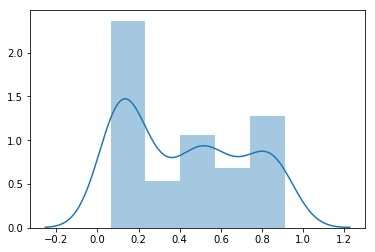
\includegraphics[width=\textwidth]{0.png}
		\caption{训练1个epoch后}
	\end{subfigure}
%%%%%%%%%%%%%%
	\begin{subfigure}{.4\textwidth}
		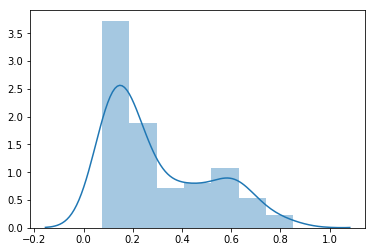
\includegraphics[width=\textwidth]{1.png}
		\caption{训练2个epoch后}
    \end{subfigure}
    \begin{subfigure}{.4\textwidth}
		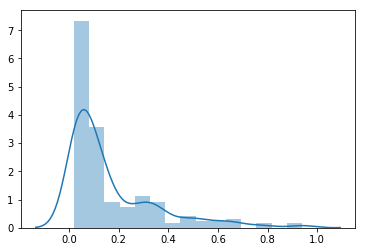
\includegraphics[width=\textwidth]{5.png}
		\caption{训练4个epoch后}
    \end{subfigure}
    \begin{subfigure}{.4\textwidth}
		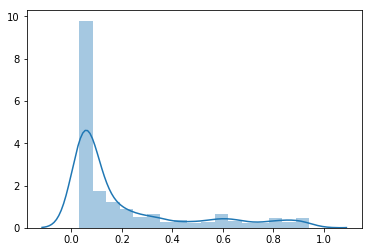
\includegraphics[width=\textwidth]{raw.png}
		\caption{真实文本的评分分布}
	\end{subfigure}
    \caption{经过数轮训练后生成序列的评分分布的变化,可以看出其越来越接近真实文本的分布}
    \label{f3-1}
    
\end{figure}
\subsubsection{生成新的事件描述}
在完成训练后,我们可以采用GAN\_PG中的生成模型来生成新的事件描述。由于使用了变分自编码器,我们只需要在隐空间中进行服从0-1高斯分布的随机采样便可以借助生成模型中的解码器来获得新的事件描述。为了减少随机性,我们还可以使用束搜索来最大化当前文本序列出现的概率。\ref{}(这里缺张表)为部分随机采样下生成的新的事件描述。可以看出其文法是通顺的,并且语义也是连贯的。

\subsection{本章小结}
本章采用了变分自编码器作为生成模型,以及上一章提出的带GRU的神经网络作为判别模型,组成了GAN\_PG。实验证明,经过训练后,GAN\_PG可以较好的生成文法通畅的事件描述,并且生成事件描述的评价分布也与真实的事件描述类似。通过在已知的事件描述周围采样,我们还能借助GAN\_PG来生成与原事件描述类似,但能够在判别模型获得更高评分的新的事件描述。这在某种程度上起到了改进事件描述的作用。
\end{document} 
